% -*- program: pdflatex -*-
\documentclass[fleqn,10pt,lineno]{wlpeerj}
\usepackage[hidelinks]{hyperref}
\usepackage[T1]{fontenc}
\usepackage{tgtermes}
\usepackage{etoolbox}
\usepackage{graphicx}
\hypersetup{
   pdftitle={CVX},
   pdfauthor={Alexa Tyszka, Karolis Ramanauskas, Boris Igi{\'c}}
   }
\usepackage[all]{hypcap}
\usepackage{doi} % remove url!
\graphicspath{{figures/}}
\renewcommand{\bibsection}{\section*{References}}
\providecommand{\e}[1]{\ensuremath{\times 10^{#1}}}
\newcommand{\ca}{\textit{ca}.}

%--------------------------------------------------
% How to Handle Supplemental Materials
%--------------------------------------------------

% PeerJ instructions:
%
% Supplemental materials. Online publishing allows inclusion of information that may not fit into a printed paper with page limits or may be deemed redundant (tables of data included in a figure) or otherwise inappropriate for the print version (extensive photographic evidence, metadata, other potentially useful information not essential to the paper). These files are not included in the page/word counts of the manuscript and will be presented online as submitted by the authors (not copy edited). Authors should upload this information as a separate file entitled ?Supplement? in PeerTrack. Text references to this material in the manuscript will be inserted as hotlinks to the online information. Supplemental figure and table numbers should be preceded by the letter S to indicate supplemental (Supplemental Table S1, Supplemental Fig. S4).
%
% Here's what we'll do:
% (1) we'll have another tex file called cvx-cactaceae-suppinfo.tex and we'll insert it for use in this file as follows:
% \externaldocument{cvx-cactaceae-suppinfo.tex}
%
% (2) each figure table will be inserted as usual with \begin{figure} ... \end{figure}
% (3) In the text, you just reference these with their label, as you would any other figure! That's it!

%--------------------------------------------------
% TITLE PAGE
%--------------------------------------------------
\title{Genome evolution, taxonomy, and transmission of potexviruses in cacti (\textit{Alphaflexiviridae})}

\author[1,$\dagger$]{Alexa Tyszka}
\author[1]{Karolis Ramanauskas}
\author[1]{Boris Igi\'c}
\affil[1]{Department of Biological Sciences, University of Illinois at Chicago, 840 West Taylor St.\ MC067, Chicago, IL 60607, United States of America}
 \affil[$\dagger$]{Author for correspondence.}


%\begin{linenumbers}
%\modulolinenumbers[1]
%\setstretch{1.0}

%--------------------------------------------------
% ABSTRACT 
%--------------------------------------------------

\begin{abstract}

% incomplete draft, but reasonable
\textit{Potexvirus} is a group of positive-sense single-stranded RNA viruses known to infect many flowering plants, including cacti (Cactaceae).
The current viral taxonomic naming schemes in this group often employ informal or outdated host plant names (synonyms), which complicate systematic study.
One such group, often named with a suffix "Virus X," presents a further complication---nearly all of its published sequences are from infections of cultivated plants, in which infections may dramatically affect yield.
Because their host-specificity is broad, the source of infections, the natural distribution of this group, and the significance of infections in wild species of cacti all remain unclear.
The lack of clarity is partly related to low sampling across the Potexviruses that infect cacti. 
And yet, the availability of sampled plant transcriptomes, all of which are practically metatranscriptomes, has recently exploded, along with the decreasing expense and difficulty of conducting RNAseq experiments.
Here, we harness these new tools and perform phylogenetic analyses aimed at clarifying taxonomic diversity, quantifying patterns of tissue expression, diversity, and examining selective pressures across viral genomes. 
The results suggest a novel mode of transmission by sex (pollination) for this viral group, based on significant expression in pollen.
We examine and discuss the implications of our key results for the taxonomy of \textit{Potexviruses} that infect Cactaceae, noting their vastly understudied ecological significance.
\end{abstract}

%--------------------------------------------------
\begin{document}
%--------------------------------------------------
%
\flushbottom
\maketitle
\thispagestyle{empty}
%\setlength{\emergencystretch}{7.5pt}
%\setstretch{1.0}
%\setlength{\parindent}{0.25in}

%--------------------------------------------------
\section*{Introduction}
%--------------------------------------------------

Molisch's (1885) \nocite{molisch1885} discovery of ``protein bodies'' on several species of cacti was one of the first documented descriptions of viruses.
For nearly a century, subsequent comparative study of viruses remained limited to direct observational data of gross morphology, augmented with clever experimental approaches, such as filtration and inoculation \citep{mettenleiter2017}.
A transformative advancement in virology---and all of biology---has been the advent of massively parallel DNA and RNA sequencing. 
The rapidly improving sequencing tools enable rapid identification of organisms from seemingly any sampled surface of the Earth.
One common thread is that virtually every macro-organism genome study uncovers a micro-organismal metagenome, composed of both targeted host sequences and those from myriad co-existing organisms. 
Metagenomic studies have yielded an enormous number of genomes and have vastly expanded the global viriome \citep{gregory_marine_2019,lefeuvre2019,shi_redefining_2016}. 
%B: this is an unusually large in-line citation set. I would pick one or two transformative studies, not the whole gamut.
The unprecedented amount of data resulting from metagenomic studies has also caused significant policy changes and revisions by the International Committee on Taxonomy of Viruses (ICTV) policy \citep{ictv2020,simmonds2017virus}, but nearly all viruses remain named by their original description of host, location, and/or symptoms.

The historic naming conventions are ill-suited for host plants whose own taxonomic placement is uncertain, which has been particularly true for rapidly diversified groups such as Cactaceae (cacti).
Molisch's ``protein bodies'' are now widely understood to be comprised of plant-infecting potexviruses (\textit{Tymovirales}, family \textit{Alphaflexiviridae}).
Their positive-sense, single-stranded RNA genomes consist of 5.9-7.0 kb of positive-sense single-stranded RNA \citep{martelli_family_2007}.
Generally presenting as elongated, rod-shaped filamentous viruses, they express five primary open reading frames (ORFs): Replicase (Rep), Triple gene block (TGB), Coat protein (CP), coded in the 5' direction as well as two smaller overlapping ORFs coded in the 3' direction: ORF6 and ORF7 \citep{martelli_family_2007}. 
%if one of these citations mentions the structure, it is sufficient.
%at: deleted all but the most relevant citation
%They are closely related to other \textit{Potexviruses} such as \textit{Alternantha Mosaic Virus} and \textit{Papaya Mosaic Virus} \citep{martelli_family_2007,park_detection_2018,liou_complete_2004}.
Members of this group produce variably symptomatic infections in cacti, and many infected plants show no external signs of viral infection \citep{bos_symptoms_1977, liou_complete_2004}. 
Neither the significance of their infections in nature, nor relative modes of transmission are clear. 
Reports of symptomatic plants range from 0\%-5.5\% in wild species in the southwestern United States \citep{attathom_occurrence_1978} to 44\% in agricultural fields on Hainan Island, China \citep{peng_molecular_2016}.
The most commonly recognized symptoms of the disease are mosaic, mottling, stunted growth, and distortion \citep{attathom_occurrence_1978, maliarenko_cactus_2013, peng_molecular_2016}.
Infection through grafting and mechanical contact, particularly following stem injury and human-mediated or hemipteran insect-mediated sap inoculation, is well-documented \citep{liou_complete_2004,maliarenko_cactus_2013,park_detection_2018}.
Grafting is a primary means of propagation among crop cacti \citep{park_detection_2018}, and \textit{Selenicereus} is a commonly chosen graft stock.
However, there are reports of other members within the family \textit{Alphaflexiviridae} transmitting via insect and seed vectors \citep{martelli_family_2007}, and pre-DNA studies tentatively suggest that in the wild, pollen may transmit \textit{CVX} \citep{attathom_occurrence_1978}.

%This paragraph needs a topic sentence: "viral taxonomy is complicated by many aspects of biology and taxonomic practices" or something.
\textit{Schlumbergera truncata} (Haworth) Moran has undergone a number of name changes, including \textit{Epiphyllum truncatum} Haworth in 1819, \textit{Cactus truncatus} (Haworth) Link in 1822, and \textit{Zygocactus truncatus} (Haworth) K. Schumann in 1890, dramatically confusing subsequent viral taxonomy.
%This naming scheme may cause confusion as it results in many distinct viruses having the same name.
Thus, currently accepted names in the \textit{Potexvirus} group include \textit{Cactus Virus X} (CVX), \textit{Zygocactus Virus X} (ZyVX), and \textit{Schlumbergera Virus X} (SchVX), each of which was likely characterized on the same host genus (and possibly species). %cite
The Baltimore classification system standardizes viral classification by intrinsic morphological characteristics of a virus' replication machinery. 
It has been integrated into the ICTV guidelines to better reflect viral evolutionary relationships \citep{ictv2020}.
The term ``plant virus'' in itself is problematic since there is strong evidence to suggest that many viruses have transitioned from fungal or invertebrate hosts to plant hosts \citep{lefeuvre_evolution_2019}. %this is possibly important and I have not read the paper. The interpretation of possibility of spillover is critical. Make sure that there are documented cases where a species jumps host across this chasm!
Additionally, many plant viruses that infect agriculturally important species are named using the common name of a plant, which carries its own problems, for example: \textit{Pitaya Virus X} is named for the common name ``Pitaya'' which can refer to as many as thirty-one species within the genus \textit{Selenicereus} \citep{korotkova_phylogenetic_2017,guerrero_phylogenetic_2019,le_bellec_12_2011}. 
The matter is further complicated by basic viral ecology, because one virus may infect many hosts, and one host may be co-infected by many viruses. 
Single-stranded RNA viruses have faster rates of evolution than their host plants. %B: just one virus is considered in this whole section?
It engages in a different mode of reproduction, making a direct assignment of viruses and their hosts difficult (citation needed).%rephrase
There is no guarantee that viral evolution and speciation follow linearly behind plant evolution and speciation---especially due to viral host-switching.
These problems persist throughout the genus \textit{Potexvirus} and are especially prominent in cactus-infecting \textit{Potexvirus} species.
We suggest a phylogeny-based approach to remedy some prominent taxonomic issues within this specific clade that cause naming inconsistencies.

%at: I will trim this down soon and make it introduction-worthy. 
%The species \textit{Cactus Virus X}, \textit{Zygocactus Virus X}, \textit{Schlumbergera Virus X}, \textit{Pitaya Virus X}, and \textit{Opuntia Virus X} are all \textit{Potexviruses} (family Alphaflexiviridae) that are grouped broadly by their infections of certain cacti: \textit{Selenicereus undatus} and \textit{S. polyrhizus} \citep{li_viral_2015,peng_molecular_2016}; \textit{Opuntia spp.} especially \textit{O. tuna} \citep{koenig_molecular_2004, duarte_Potexvirus_2008} and \textit{O. monacantha} \citep{attathom_occurrence_1978} Sammons 1961 Duarte 2008; \textit{Schlumbergera} (previously \textit{Zygocactus}) \textit{truncata} and \textit{S. bridgesii} \citep{duarte_Potexvirus_2008, koenig_molecular_2004}, \textit{Parodia }(previously \textit{Notocactus}) \textit{leninghausii} \citep{park_detection_2018}, \textit{Echinopsis chamaecereus f. cristata}, \textit{E. pectinatus f. cristata}, \textit{E. jusbertii}, and \textit{E. macrogona} \citep{maliarenko_cactus_2013}; \textit{Mammillaria elongata f. cristata} \citep{maliarenko_cactus_2013}; and multiple other species within many genera in the family Cactaceae \citep{evallo_brief_2021}. Of these viruses, only \textit{Cactus Virus X} (CVX) has been reported on wild \textit{Ferocactus cylindraceus} (previously \textit{Ferrocactus acanthodes}) \citep{attathom_occurrence_1978}. 
%However, this report predates DNA records confirming the viral identity.
%Additionally, the viruses are frequently manipulated with serological experiments and have been found to produce lesions (which indicate infection) on: \textit{Chenopodium murale L.} \citep{maliarenko_cactus_2013} and C. quinoa \citep{attathom_identification_1978,attathom_occurrence_1978, brandes_untersuchungen_1963-1}; Nicotiana alata Link el. Otto \citep{maliarenko_cactus_2013}; Four species of Amaranthaceae \citep{attathom_identification_1978}; Escobaria vivipara \citep{attathom_identification_1978}; and other Cactaceae \citep{attathom_identification_1978}.

Knowledge about cactus-infecting \textit{Potexviruses} contributes to a growing yet biased study of plant viruses. 
Human-assisted dispersal, grafting, and cultivation obscures the evolutionary history of these viruses, which parallels the disproportionate sampling representation of plants raised in greenhouses or for agricultural production. 
However, \textit{Cactus Virus X} and associated viruses seem restricted to cactaceous hosts for unknown reasons---every sample of CVX or CVX-related viruses has come from cacti.
The few studies that have investigated wild \textit{Potexviruses} of cacti predate DNA methods and have yet to identify the origin.
Recent sequencing efforts have revealed multiple inconsistent virus-host pairs on cacti.
Although many metagenomic studies capture environmental, genetic information that allows for virus identification, tissue type may bias expression rates of viruses \citep{lacroix2016methodological}.
The pursuit of wild cactus-infecting \textit{Potexviruses} expands our evolutionary knowledge of viral evolution, host selection, and transmission mechanics. 
The relationships of the virus can be investigated with a thorough phylogenetic approach, using available virus samples. 
In this study we present the largest to date phylogeny of cactus-infecting \textit{Potexviruses}.
We attempt to use this expanded phylogeny to answer relevant questions about Potexvirus evolutionary relationships and revisit the utility of decades-old taxonomy in current virus research. 


% METHODS ====================================================================
%------------------------------------------------------------------------------
\section*{Materials and Methods}
%------------------------------------------------------------------------------

\subsection*{Host Study Species}

We relied on two types of sequencing data for all analyses: original sequences obtained from tissues we collected and sequences deposited in public sequence data archives. 
We recovered original viral sequence data from tissues of \textit{Schlumbergera truncata} (Haworth) Moran, commonly known as ``crab cactus'' or ``false Christmas cactus,'' a widely cultivated species.
Although there are dozens of named varieties of this species, nearly all commercially grown plants are of uncertain provenance. 
They almost certainly trace to a handful of plants collected in their native Atlantic forests of Brazil and brought to England in the early 1800s \citep{boyle2003}. 
Plants are easily grown from cuttings and the species has been extensively hybridized across Western Europe and exported across the world, prized for their showy winter (short-day) displays.
Our host plant samples were sourced from a haphazardly collected personal collection (B.I.), purchased or found abandoned around the city of Chicago. 
Most of the plants were either apparently asymptomatic or weakly symptomatic at the time of tissue collection.
All of our accessioned host plants are independent genets (unique genotypes) \citep{ramanauskas2021}.
%refer to (supplementary?) table 1 with accessions and sequencing 

\subsection*{RNA Sequencing}

Pistils (without ovaries), pollen, leaf, and root tissues were removed and submerged in 1.5 ml of $RNA\textit{later}{\texttrademark}$ solution (Invitrogen).
Samples were held at room temperature for 30-60 minutes and then moved to a -80 C freezer for storage.
Approximately 100 mg of tissue was ground to a fine powder in 1.5 ml tubes submerged in liquid nitrogen.
Total RNA was isolated using Total RNA Mini Kit (Plant kit; IBI Scientific, Cat. No. IB47341) following manufacturer's instructions.
We assessed RNA concentration and purity with a NanoDrop\texttrademark~Lite Spectrophotometer (Thermo Scientific).
%FIXME: time to get rid of XXX everywhere.
The XXX samples used in this study were sequenced as part of a larger sequencing effort which consisted of XXX separate sequencing runs and included additional samples from other plant species.
Sequencing libraries were prepared using the KAPA Stranded mRNA-Seq (Roche)
These libraries were sequenced on a single lane of Illumina \mbox{HiSeq}~4000 or Illumina \mbox{NovaSeq}~6000 platform (paired-end 150 bp reads) at the Duke University Center for Genomic and Computational Biology.
The number of resulting read pairs (for the XX samples presented here) ranged from X,XXX,XXX to X,XXX,XXX with a median of X,XXX,XXX and average of X,XXX,XXX (Table~S1).

\subsubsection*{RNAseq from deposited sequence read archives}

We searched the NCBI Sequence Read Archive (SRA) database (www.ncbi.nlm.nih.gov/sra) for RNA-sequencing (RNA-seq) data within the flowering plant order Caryophyllales (NCBI:txid3524) that had been sequenced using an Illumina library sequencing platform. 
For each identified SRA run accession (SRR), viral RNA that matched sample cactus-infecting Potexvirus RNA (accession numbers provided in Supplemental Information ) was identified, extracted, and assembled using the kakapo 0.7.3-dev pipeline (http://flightless.one) with Kraken2 viral filters disabled. 
The search returned 59 sequences aligned to members of Potexvirus within PRJNA608981 (https://www.ncbi.nlm.nih.gov/Traces/study/?acc=PRJNA608981).

Additional publicly available partial or complete viral genomes, gene annotations, and available metadata from Potexviruses (NCBI:txid12176) were downloaded from NCBI (NCBI: www.ncbi.nlm.nih.gov/, accession numbers provided in Supplemental Information).
We obtained host information through NCBI reported metadata.

\subsection*{RNAseq Assemblies}

Raw paired-end Illumina reads were first processed using \mbox{Rcorrector}~v1.0.4 \citep{song2015} to infer and correct sequencing errors.
Reads were next trimmed with \mbox{Trimmomatic}~v0.39 \citep{bolger2014} to remove any read containing bases with Phred scores lower than 20, low quality reads less than 50 bp long, and any adapter or other Illumina-specific sequences that were still present.
The remaining reads were filtered with \mbox{Kraken}~2 \citep{wood2019} to remove small and large subunit ribosomal RNA (using the SILVA database; \citealt{quast2013}) and contaminating reads (minikraken2\_v2 database).
We used custom-built databases, derived from RefSeq libraries: UniVec\_Core, viral, mitochondrion, plastid, plasmid, archaea, bacteria, protozoa, human, and fungi to minimize the number of contaminating and non-nuclear reads \citep{ramanauskas2021}.
Only paired reads were used for transcriptome assemblies.
\textit{Schlumbergera truncata} filtered reads were combined across all samples into a single RNA-seq data set.
We conducted a \textit{de novo} transcriptome assembly using \mbox{Trinity}~v2.8.5 \citep{grabherr2011} 
to generate a single reference transcriptome assembly for \textit{Schlumbergera truncata}.

\subsection*{Sequence Alignment and Phylogenetic Analyses}
The untranslated regions (UTRs) were trimmed from the sequences for consistency.
Sequence alignments were performed through MAFFT v7.429 \citep{katoh_mafft_2002} using the full dataset.
%FIXME: MAFFT settings/options missing. DNA or protein? (These Methods paragraphs should be detailed.)

The aligned sequences were divided by ORF using annotations to produce sequence alignments for each of the five genes, along with the whole-genome alignment. 
The individual proteins were exported to FASTA files, then gaps at the start of the sequence and stop codons were removed manually. 

%FIXME: this previously read "v1.6.12" \citep{nguyen2015}., which seems incorrect, according to genbank_kr_consensus_extraction_al_trimmed.fasta.iqtree. 
%also, %B: I went through some files and found several iq-tree files. I assume that the latest one, genbank_kr_consensus_extraction_al_trimmed.fasta.iqtree is the correct one. If the others are not being used, they should be deleted from the shared git archive.
%at: removed old fasta files from repo
Phylogenetic relationships, including those used for assessing bootstrap support, were inferred using \texttt{IQ-Tree} v2.0.3. 
Maximum likelihood inference for the whole genome sequences---as well as for each gene region, separately---relied on a model of sequence evolution (GTR+F+I+$\Gamma$4) favored by both AIC- and BIC-based selection procedure implemented in IQ-Tree's model selection module {\em ModelFinder} \citep{kalyaanamoorthy2017}. Akaike and Bayesian weights exceeded 0.99. 
%put in Results--if true: We also implemented an identical analysis for each of five genes, separately, but the results are virtually identical.
%at: We have AIC scores for the rest of them, but I did not run modelfinder on each. I can rerun it if needed.
Branch support was assessed with IQ-Tree's {\em UFBoot}, an ultrafast bootstrap implementation \citep{hoang2018}.


% FIXME: No mention why Sequence Percent is calculated. ICTV rules? What is done with  alignment gaps?
% at: mentioned ictv.
\subsubsection*{Sequence percent identity calculation}
ICTV guidelines state that species within\textit{Potexvirus} are delineated by 72\% shared nucleotide identity, or 80\% shared amino acid identity within the coat protein or replication genes. 
Percentage sequence distance was calculated for Coat Protein (CP) and RdRp nucleotides and amino acids using SDT v1.2. %FIXME version missing (at:fixed)
In cases where the CP and RdRp nt sequence distances fell on opposite sides of the 72\% cutoff, the disagreement was noted.
Sequences with partial CP or RdRp genes were removed from the disagreement calculations to avoid length-based false positives. %post-analysis? If it is after the analyses? If so, it seems to be not used in analyses, which is odd. I think you mean after some of the analyses before others, maybe. Detailed description missing.
%at: fixed, potentially.
For each defined clade, nonzero pairwise distances between each possible combination of tips was averaged. 
Raw pairwise distance analysis was conducted on the sequence alignments in R using \texttt{ape} v5.5.
\subsubsection*{Analysis of molecular selection}

\subsection*{Data Accessibility}

This article contains a Supplementary Information Appendix. %What's in it?
 %Is it Supplementary Information Appendix or Supplementary Data?
 %at: changed references to all be Supplemental Information for consistency
All new sequence data is deposited in GenBank under project accession number PRJNXXXXX (https://www.ncbi.nlm.nih.gov/Traces/study/?acc=PRJNXXXXX). %Not all? specifically, it's the schlumbergera data, right? Which ones?
%at: should the data be deposited with any reference to CVX, or is just referring to the schlumbergera data SRAs okay in this case?


%------------------------------------------------------------------------------
\section*{Results}
%------------------------------------------------------------------------------
\subsection*{Viral Identification}
In an attempt to characterize the infection patterns of cactus-infecting potexviruses, we assembled 69 viral sequences from the XXX total cactus samples analyzed (Table 1).
%FIXME: noauthor?
The genome sizes of 6.6-6.7 kb were consistent with ICTV reported 5.9-7.0 kb genome lengths within \textit{Potexvirus} \citep{noauthor_genus_2020}.
In some cases, one cactus sample contained multiple different virus species (Table 1).

%FIXME: is this a method or a result? And what is the method or result being reported? What was the content of annotation?
We annotated the open reading frames of the viruses and recovered all Potexvirus proteins.

\subsection*{Phylogenetic Relationships}
A well-supported phylogenetic tree was recovered using available sequences (Figure 1).
The 69 viral sequences were in some cases concatenated for ease of viewing on the tree.
The phylogenetic tree places the newly aligned sequences from this study within previously defined species groups (Figure 1).
These sequences greatly expand the cactus-infecting clade of \textit{Potexvirus} by a roughly XXX percent increase. 
Phylogenetic analysis recovered defined monophyletic groups corresponding to five or six major groups of cactus-infecting \textit{Potexviruses}, with \textit{Cactus Virus X} displaying two branching subgroups.
\textit{Opuntia Virus X} was the sister clade to the rest of the cactus-infecting \textit{Potexviruses}.
We recovered viruses within the Potexvirus clades: \textit{Cactus Virus X, Pitaya Virus X, Schlumbergera Virus X}, and \textit{Zygocactus Virus X} (Table 1).
Bootstrap values 

\subsection*{Species Delineation and Distribution of Genetic Distances}
Graphical representation of nonzero raw sequence distances is provided in Figure 1b. 

\subsection*{Infection Prevalence and Symptoms}
The \textit{Schlumbergera}-infecting viruses were found in high amounts on pollen and style tissue (Table 2).
In some pollen tissues there existed more viral reads than \textit{Schlumbergera} reads.

The \textit{S. truncata }samples located within the \textit{Cactus Virus X} clade appear to represent the first known discovery of \textit{Cactus Virus X} on \textit{Schlumbergera}.
Host information, collected from available metadata, shows several different host genera for any one virus (Figure 1).
PRJNXXX did not report plants as symptomatic or asymptomatic, and did not report 
 
\subsection*{Recombination Analysis and Selection Analysis}
The gene trees recovered for the five major \textit{Potexvirus} proteins (\textit{CP, RdRp, TGB1, TGB2, \textit{and}TGB3}) retained the species groupings shown by the full genome tree, which indicates low levels of gene conflict (Figure 1S).


%------------------------------------------------------------------------------
\section*{Discussion}
%------------------------------------------------------------------------------
Cactus-infecting potexviruses present an evolutionary puzzle as well as an agricultural threat. 
In this study we use a multiple-source transcriptomic approach to address the questions of \textit{Potexvirus} host specificity and evolution. 
We present another use for the \textit{kakapo} program: effective, fast search and assembly of small viral genomes rather than individual genes. 
We detected viral samples that were phylogenetically related to four current species within \textit{Potexvirus}: \textit{Cactus Virus X, Schlumbergera Virus X, Pitaya Virus X}, and \textit{Zygocactus Virus X}. 
Within \textit{Cactus Virus X}, there may be reason to delegate two subspecies or split the species altogether. 
We offer a further discussion regarding erroneous viral taxonomy and nomenclature within the current metagenomic era.

A well-supported phylogenetic tree was recovered including closely related non-cactus-infecting \textit{Potexviruses} as an outgroup (Figure 1).
The phylogenetic tree (Figure 1) places the new viral sequences found on hosts \textit{Schlumbergera} and \textit{Selenicereus} near existing viral species within \textit{Potexvirus} (Figure 1). 
The newly reported infections represent new examples of \textit{Cactus Virus X, Schlumbergera Virus X, Pitaya Virus X}, and \textit{Zygocactus Virus X}.
Some closely clustered examples likely represent one primary infection spreading to multiple plants due to the extremely low within-clade diversity (Table 1).
For this analysis we refer to the two branches of\textit{ Cactus Virus X }as \textit{Cactus Virus X A} and \textit{Cactus Virus X B} because the formal taxonomic group \textit{CVX} was the only group distinguished by high p-distance values (Full sequence mean 0.0399; RdRp mean 0.0343; CP mean 0.0453) as well as a notable bifurcation within the group (Figure 1).


The origins of 0.72 difference --- clade delineation --- summary of infections and hosts --- multiple infections --- relation to other studies --- success of testing --- naming complications --- names using in paper --- history of naming conflicts --- recommendations for future --- identification/infections --- often symptomless confused for other diseases --- extent yet unknown --- further obscured by species delimitations --- distinguish between infection and transmission because in this case infection may not always lead to transmission. 

Most experimental transmission of cactus viruses is done in a manner that would rarely be reproduced in the field under natural conditions --- grafting  is frequent in greenhouses, inoculation and transmission --- transmission methods --- review of other papers? --- thesis, saguaro nectar --- relation to sexual transmission
 
The reported taxonomy of each existing sample aligns well with the tree structure, but this monophyly is not recovered for hosts.
Putative viral species appear to infect as few as one genus, in the case of \textit{Opuntia Virus X}, or as many as three in the case of \textit{Schlumbergera Virus X}.
Further, the three genera are evolutionarily distinct and polyphyletic in phylogenetic analyses of \textit{Cactaceae}. 
This relationship raises questions about a \textit{Potexvirus}'s ability to switch hosts. %clarify
All three genera that are reported hosts of \textit{Schlumbergera Virus X} are ornamental crops: \textit{Selenicereus, Schlumbergera}, and \textit{Opuntia}.
Extended greenhouse contact between the three genera may have resulted in viral spillover of \textit{Schlumbergera Virus X}.
However, it is also important to note that the present viral taxonomy is not infallible. 
The putative species known as \textit{Schlumbergera Virus X} may have been initially - incidentally - found on a spillover host rather than a member of an actual viral circulating population.
Unfortunately there is no way to know the "original host" of any virus that possesses the mechanisms to infect multiple cacti genera. 
Further testing of known host genera is necessary, and metagenomic sequencing of closely related genera to monitor potential opportunistic spillover. 

Taxonomic descriptions must also be analyzed for accuracy and reflection of actual viral activity. 
A virus named for its first known host may not represent the evolutionary history of the virus.
Although phylogenetic analysis is likely to produce monophyletic clades of viruses that have each been named in succession for the first known member, this produces inconsistent and confusing names.
\textit{Zygocactus Virus X} is a clear example: Although the name \textit{Zygocactus} is outdated in reference to the host genera, now classified as \textit{Schlumbergera}, the viral name remains.
This is exacerbated by the presence of a separate viral species, \textit{Schlumbergera Virus X}.
The ICTV strongly opposes unnecessary name changes, but it is unclear what should be done with outdated and confusing names that describe an extant clade of viruses.
Mixed infections and the lack of a one-to-one correlation between virus and host complicate naming endeavors further, and more sampling will uncover novel hosts and mixed infections.

\subsection*{Distribution of Genetic Distances and Grouping}
The highly similar and well-clustered newly discovered viruses displayed low diversity within the clusters (Figure 1b).
Therefore, these additions to the \textit{Potexvirus} family tree do not drastically alter the tree structure.
Since each sampled cactus in SRA XXXXX was located close to other sampled cacti, this low diversity potentially represents the first example of background mutation among viruses incurred due to host infection.


The ICTV guidelines for \textit{Potexviruses} indicate that less than 72 percent nucleotide sequence identity (or 80 percent amino acid identity) between the CP or Rep genes demarcates separate viral species. %clarify 
Because we compare closely related \textit{Potexviruses}, it might be expected that members of the same putative species would have higher than 72 percent nucleotide identity and members of different putative species would have lower than 72 percent sequence identity.
However, the low pairwise distances between \textit{Potexviruses} cause very few cactus-infecting \textit{Potexviruses} to be demarcated as separate species, even when only considering previously described species compared to each other.
Examples here.

\section*{Conclusions}
X new viruses were included as part of this study, which represents a multifaceted approach to viral discovery using metagenomic techniques for already available public data as well as newly collected data.
Mixed infections, co-infection dynamics.
Viral abundance, viral loads, tissue type, and diversity.
Transmission: Sexual
Taxonomic recommendations - the current species names should not be used in the future.
%------------------------------------------------------------------------------
\section*{Acknowledgments}
%------------------------------------------------------------------------------

This work was supported by the Award for Graduate Research from the Graduate College, University of Illinois at Chicago (to K.R.) and the National Science Foundation grant NSF-DEB-1655692 (to B.I.).

%--------------------------------------------------
% References
%--------------------------------------------------
\clearpage
%\raggedright{}
%\setstretch{1.0}
%\setlength{\parindent}{0.0in}
%\bibliographystyle{evolution}
%{\fontsize{10pt}{15pt}\selectfont}
\bibliography{cvx-refs}
%}
%\end{linenumbers}

%--------------------------------------------------
% Tables
%--------------------------------------------------

%--------------------------------------------------
% Figures
%--------------------------------------------------

\pagebreak
\frenchspacing
%\setstretch{1.0}
\setlength{\parindent}{0.0in}

\section*{Figures}
Figure inventory list.



\begin{figure}[ht]
\centering
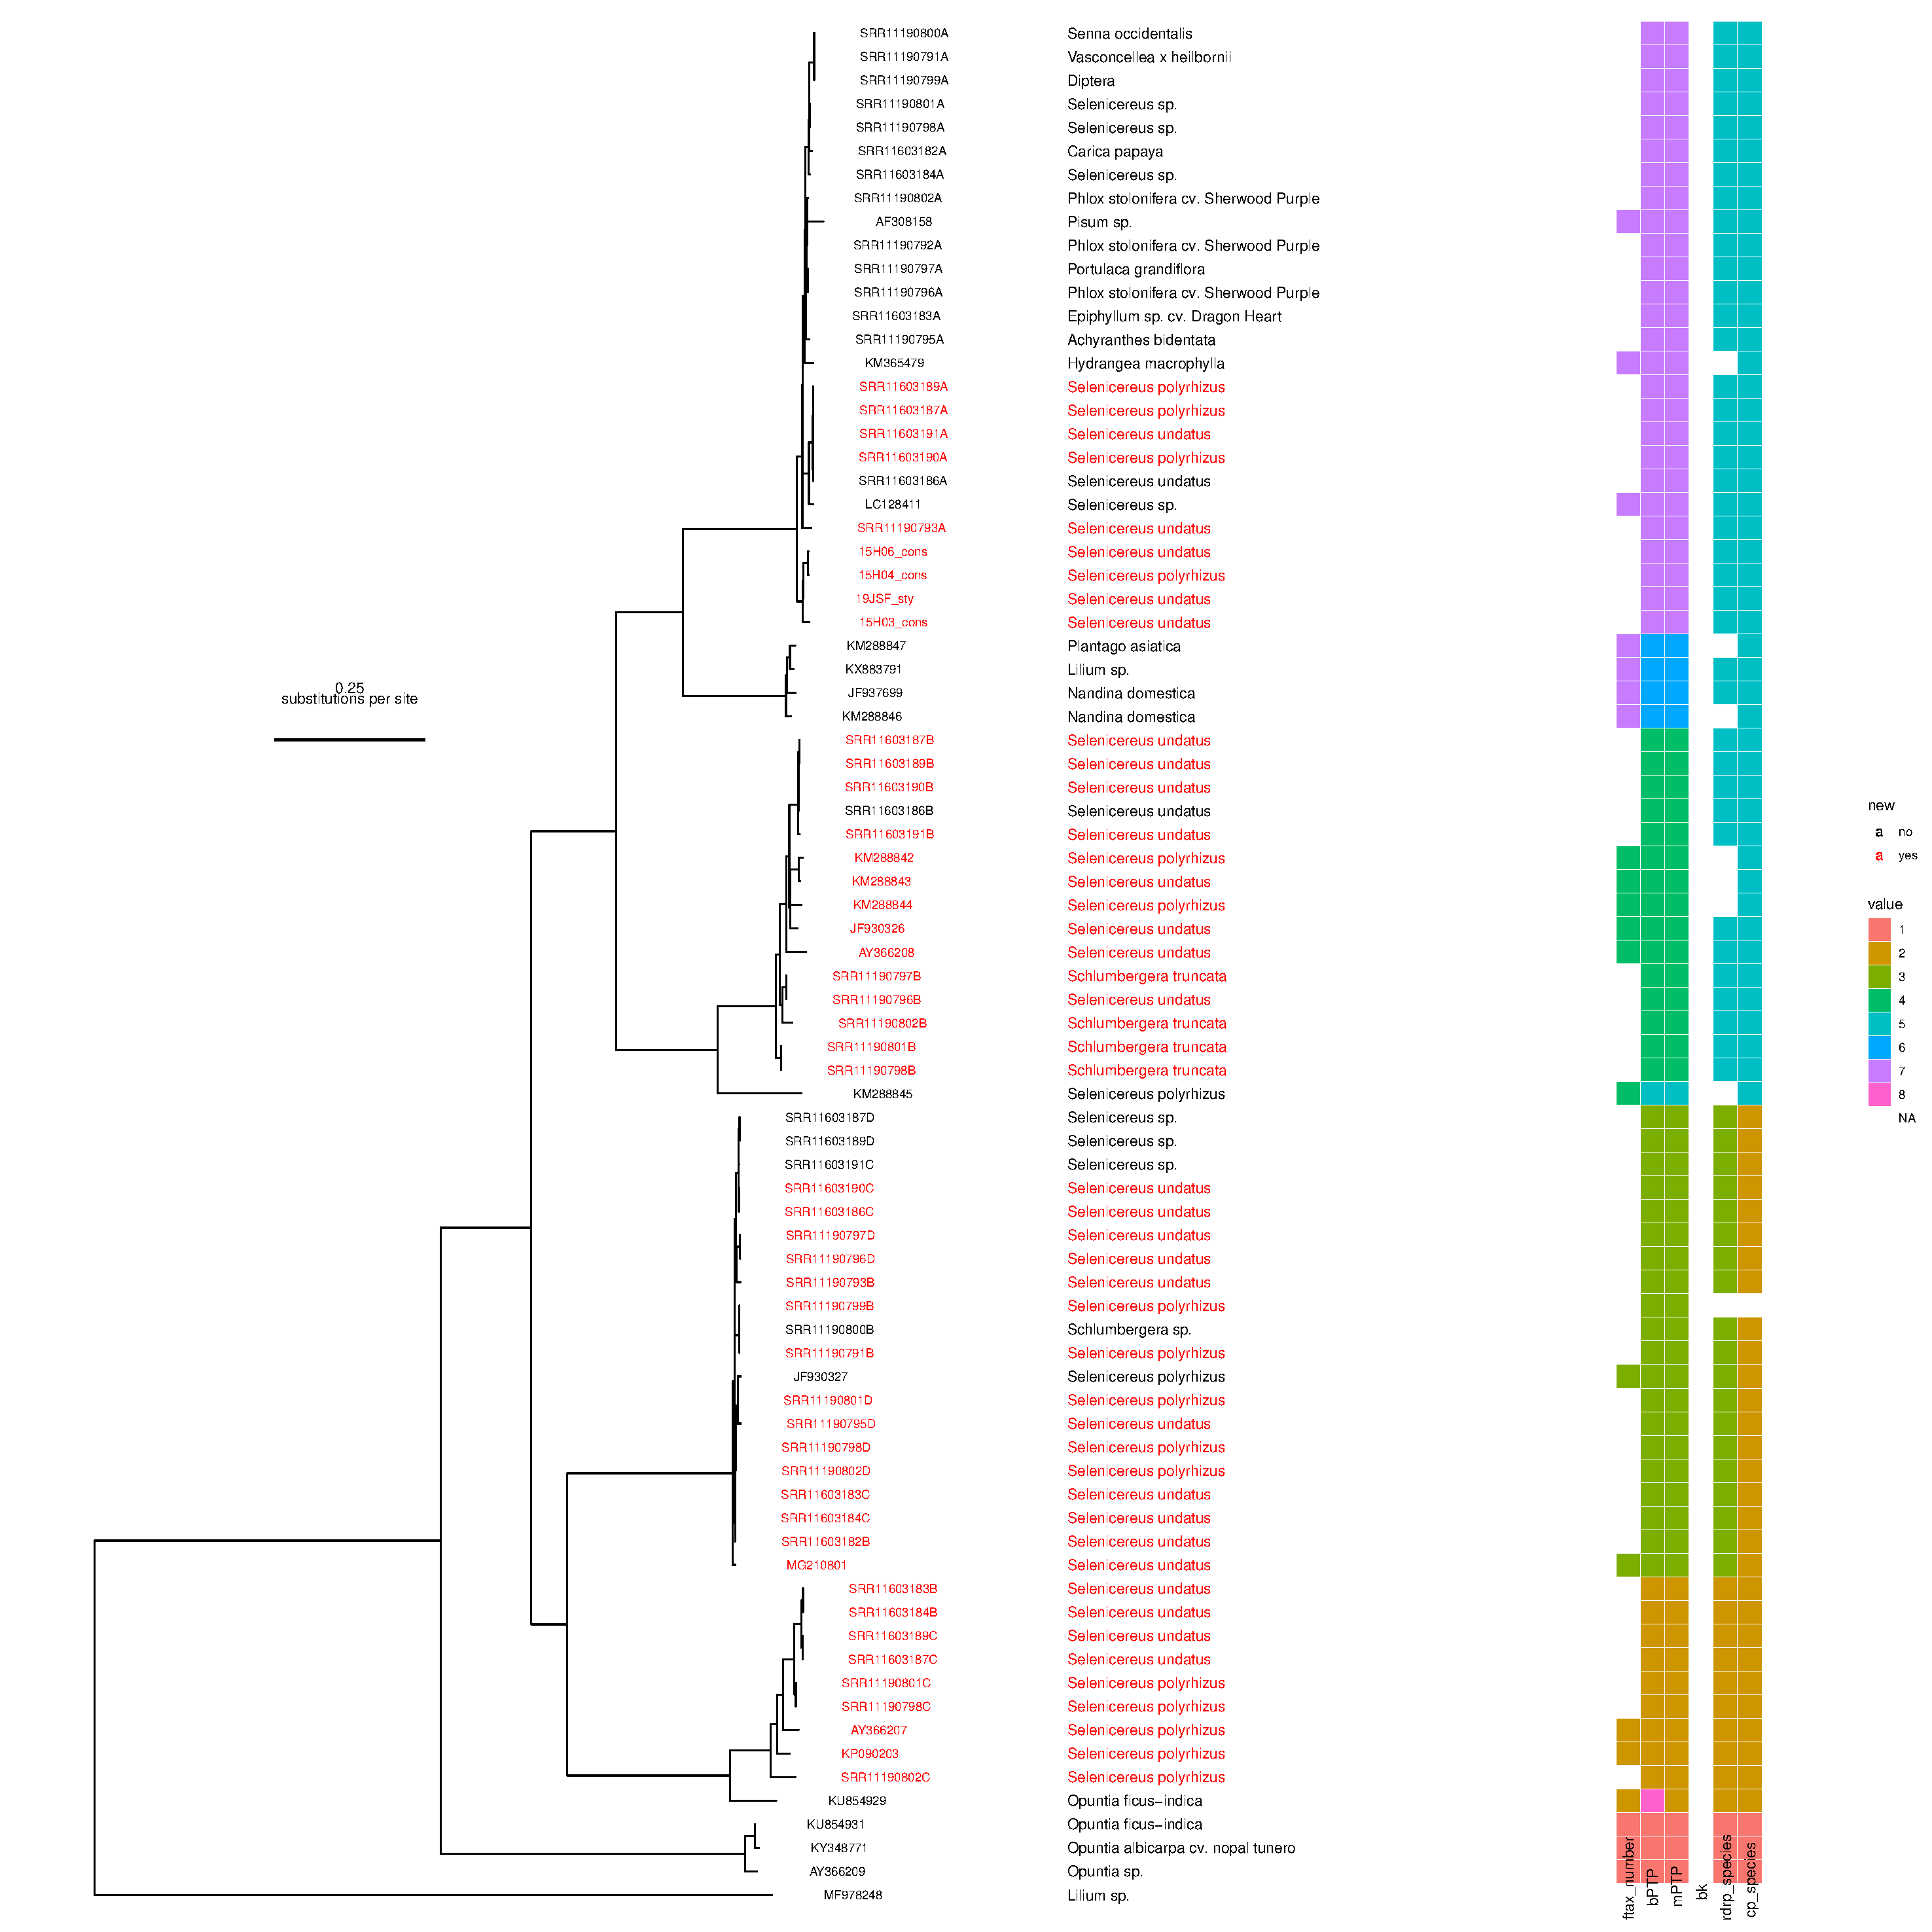
\includegraphics[width=1\linewidth]{figures/tree_rect_new_collapsed.pdf}
 \begin{NoHyper}
 \caption{The updated cactus-infecting \textit{potexvirus} phylogeny reflects distinct viral groupings which opportunistically infect multiple host plants. 94 virus sequences were aligned with MAFFT and a phylogeny was generated with IQtree. All major (clade-delimiting) nodes have greater than 95 percent bootstrap support.}
 \label{fig1}
 \end{NoHyper}
 \end{figure}
 
 Figure 1b. Genome organization outline, genome length when assembled, genome structure
 Figure 1c. columns with labels.

Table 1. Assembly stats. our taxa, SRAs, assembly stats for positive finds, including unique ID and sample names, including length

Table 2. Points under positive selection, how many in each gene


Figure 2. Selection graph as displayed in B's r code

Figure 3. (maybe supplemental) density of cp, rdrp, distributions density by virus ptp


Supplementary Table 1. All searches, cleaned SraRunInfo.csv plus KR's schlumbergera searches


Supplemental figures:
1. Full gene phylogenies for each gene in genome
2. Tissue expression rates? TMM/TPM


% \begin{figure}[ht]
% \centering
% \includegraphics[width=0.5\linewidth]{FILE_PATH}
% \begin{NoHyper}
% \caption{{\fontsize{10pt}{11pt}\selectfont}
% \label{fig:FIG_LABEL}
% \end{NoHyper}
% \end{figure}

% END =========================================================================

\end{document}
